\documentclass[letterpaper,11pt,leqno]{article}
\usepackage{../../style/paper}
\usepackage{tikz}
\usetikzlibrary{positioning}
\bibliographystyle{../../style/paper}

% Enter paper title to populate PDF metadata:
\hypersetup{pdftitle={Lacamas Watershed Council Upper Watershed Committee}}

% Enter path to BibTeX file with references:
\newcommand{\bib}{paper.bib}

% Enter path to PDF file with figures:
\newcommand{\pdf}{figures.pdf}

\begin{document}

% Enter title:
\title{Lacamas Watershed Council Upper Watershed Committee}

% Enter authors:
\author{Lacamas Watershed Council}
%
% Enter affiliations and acknowledgements:
% \thanks{First Author: First University. Second Author: Second University. We thank colleagues for helpful comments and discussions. This work was supported by a grant [grant number]; another grant [grant number]; and a foundation.}}

% Enter date:
\date{July, 2026}   

% Enter paper URL (can be commented out):
% \paperurl{https://github.com/pmichaillat/latex-paper}

\begin{titlepage}
\maketitle

% Enter abstract:

\end{titlepage}

% Enter main text:
\section{Executive Summary}\label{s:ExecutiveSummary}

\paragraph{Purpose} The purpose of this document is to establish the operational framework for the Upper Watershed Committee.
The committee will oversee all LWC efforts in the Lacamas Creek 
watershed upstream from the confluence of Lacamas Creek and Lacamas Lake \footnote{hereafter referred to as the "upper watershed"}.
This document will also establish the budget for the committee and individual upper watershed projects. Also included is a description
of volunteer positions, and the process for amending and updating this living document.

\paragraph{Goals} The goals of the upper watershed efforts are to restore the upper watershed to a healthy, nutrient-absorbing ecosystem that supports
native plant, animal, and insect species. As recommended by Washington Department of Ecology, this will be achieved by reducing nutrient pollution in streams, restoring riparian habitats, increasing shade and dissolved oxygen,
and raising awareness among stakeholders about reducing their impact on the watershed.

\paragraph{Committee Overview} To achieve the goals above, the Upper Watershed Committee will be led by a committee chair
who has liberty to recruit volunteers, use LWC resources and equipment within the approved committee budget, be a point of contact with partner organizations and landowners,
and be able to make recommendations to the board on how best to achieve the committee's goals. The committee chair will give a status report at monthly meetings and be responsible for an
end-of-season report to the board.

Within the committee, there will be a number of projects, each led by a project manager. Some are already underway. The Upper Watershed Committee is not intended to supplant the existing projects, but rather to unify them under one organizational unit. These projects will continue to operate as they have been, but will see additional organization, volunteer recruitment, and financial support.

\paragraph{Current Projects} Active projects in the upper watershed are the macroinvertebrate study and phosphate testing. The current project managers for these projects are
Rodger Hauge and Paul Witacre, respectively. A project in active development is the riparian restoration project. This is being designed collaboratively between the LWC and Clark Conservation District (CCD).

\paragraph{Adding projects} Additional projects can be added to the Upper Watershed Committee under the supervision of the committee chair. These projects may be initiated by the chair
to achieve a specific goal, or they may be initiated at the request of the board or the LWC's science advisor. Either way, all projects need to be approved by the board via the amendment process described in this document and assigned a specific project manager.

\paragraph{Budget} The total annual budget for the committee is \$5,100. A full breakdown of budget allocation is provided in this document. The appropriation that funds this budget is described in Section~\ref{s:approval}.

\section{Approval}\label{s:approval}
After deliberation the board will appoint a committee chair and vote to approve this document along with any amendments. Approving this document funds the committee for the amount of \$7,225 through December 31, 2027. That includes a prorated amount of \$2,125 for August through December 2026 and the full annual budget of \$5,100 for 2027. The funds shall be appropriated from the LWC's general fund. The \$2,125 for 2026 shall be available to the committee upon approval of this document, and the \$5,100 for 2027 shall be available on January 1, 2027.

The appropriation of \$7,225 is a ceiling on what the committee may draw from the general fund, not a commitment to spend it. Any increase to the committee's budget, including a budget for the macroinvertebrate study or the budget for any project added under Section 4, requires a separate appropriation approved by the board and shall not draw on the general fund until that appropriation is approved. Any appropriated funds that remain unspent on December 31, 2027 shall return to the general fund and shall not carry over. Funding the committee beyond December 31, 2027 requires a new appropriation approved by the board.

This appropriation authorizes the committee to incur expenses within its budget; it does not give the committee chair or any project manager custody of LWC funds. Per LWC Bylaws Article 5.5, all funds remain in the custody of the Treasurer, and all disbursements against this appropriation remain subject to the signature requirements of Article 9.3.

\section{Organizational Structure}\label{s:org}

\subsection{Upper Watershed Committee Goals}
The goal of the Upper Watershed Committee is to restore the upper watershed to a healthy, nutrient-absorbing ecosystem that supports
native plant, animal, and insect species. As recommended by Washington Department of Ecology, this will be achieved by reducing nutrient pollution in streams, restoring riparian habitats, increasing shade and dissolved oxygen,
and raising awareness among stakeholders about reducing their impact on the watershed. Reducing nutrient pollution in the upper watershed directly supports the LWC's core mission of improving the safety, health, and recreational values of the Lacamas Creek Watershed lakes.

As the committee progresses and evolves, the goals of the committee will be assessed at least annually and, where necessary, amended through the process described in Section 4 to implement the latest scientific findings and best practices. The committee chair is responsible for initiating this annual review and presenting findings to the board. The goals of the Upper Watershed Committee
shall never contradict the overall mission or goals of the LWC.

\subsection{Overview of Committee Structure}
To achieve these goals, all projects pertaining to the upper watershed will be unified under one committee within the LWC.
This will help break down the overall goal of restoring the upper watershed into smaller pieces that can be achieved by specific projects.
The committee chair is appointed by the board. Per LWC Bylaws Article 7.2, the committee must include at least two Directors; the board will designate at least one additional board member to the committee at the time of the committee chair's appointment. The committee chair must be a board member and must remain so throughout their tenure. If the committee chair ceases to be a board member, they must relinquish the committee chair role, and the board will appoint a replacement at the next board meeting. Until a replacement is appointed, the board president will assume the committee chair's responsibilities on an interim basis. Each project within the committee will be led by a project manager who reports to the committee chair.
Project managers are encouraged to attend board meetings, but this is not a requirement. Volunteers, ideally, are separated into their respective projects, but in practice they may assist with multiple projects.

\begin{center}
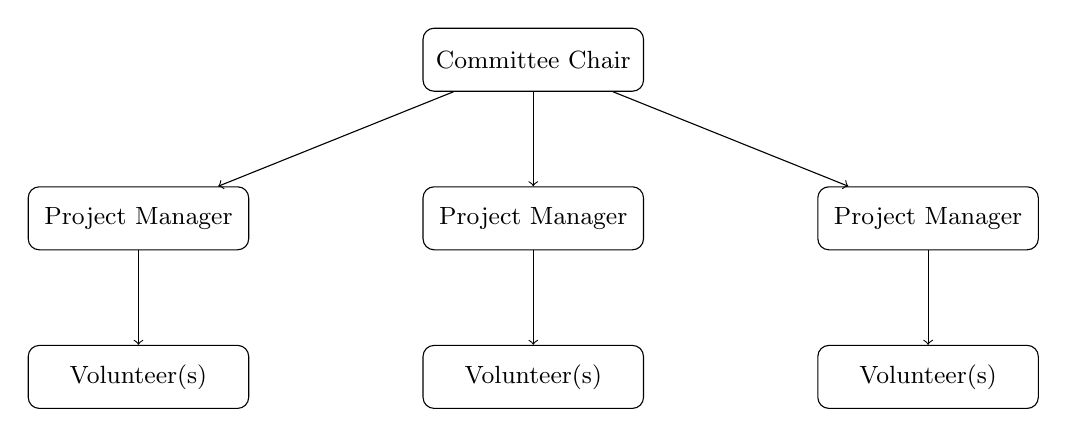
\begin{tikzpicture}[
  node distance=1.2cm and 2.2cm,
  box/.style={draw, rounded corners, minimum width=2.8cm, minimum height=0.8cm, align=center, font=\small}
]
  \node[box] (director) {Committee Chair};
  \node[box, below=of director] (pm1) {Project Manager};
  \node[box, left=of pm1] (pm0) {Project Manager};
  \node[box, right=of pm1] (pm2) {Project Manager};
  \node[box, below=of pm0] (v0) {Volunteer(s)};
  \node[box, below=of pm1] (v1) {Volunteer(s)};
  \node[box, below=of pm2] (v2) {Volunteer(s)};

  \draw[->] (director) -- (pm0);
  \draw[->] (director) -- (pm1);
  \draw[->] (director) -- (pm2);
  \draw[->] (pm0) -- (v0);
  \draw[->] (pm1) -- (v1);
  \draw[->] (pm2) -- (v2);
\end{tikzpicture}
\end{center}


\subsection{Personnel}

\subsubsection{Committee Chair}

The committee chair oversees all projects pertaining to the upper watershed. As a board member, the committee chair is responsible for
communication of board decisions to project managers, and communication of project updates and needs to the board. The duties of the committee chair include, but are not limited to, the following:
\begin{itemize}
\item Coordinate with project managers to ensure they have the correct resources for each day of fieldwork.
\item Request funding from the board and manage the committee's budget.
\item Provide monthly updates at board meetings.
\item Communicate with partner organizations and stakeholders.
\item Recruit volunteers for projects as needed.
\item Handle administrative tasks such as scheduling meetings, writing reports, and maintaining records of expenses and volunteer hours.
\item Compile and present an end-of-season report to the board at the end of each season.
\end{itemize}


\subsubsection{Project Manager}
The project manager is responsible for leading specific project(s) within the Upper Watershed Committee. Each project aims to achieve a goal or goals
of the committee, and the project manager ensures that progress is made toward those goals. The project manager also serves as a lead in the field,
ensuring successful fieldwork. They provide expertise, guidance, and volunteer supervision. The duties of the project manager include, but are not limited to, the following:
\begin{itemize}
\item Plan and lead fieldwork for the project, ensuring that all volunteers are properly trained and equipped for the tasks at hand.
\item Communicate with the committee chair regarding project needs, progress, and any issues that arise.
\item Coordinate with the LWC's science advisor to ensure that the project is following scientific best practices.
\item Compile data and report findings to the committee chair. Review the committee chair's reports and make suggestions to ensure accuracy.
\item Perform fieldwork as needed, such as collecting samples, planting trees, or maintaining restoration sites.
\item Coordinate with partner organizations and stakeholders as needed for the project. For example, working with landowners to obtain access to sites. 
\end{itemize}

\subsubsection{On-call Volunteer}
Uniquely, this committee will require a pool of "on-call" volunteers who are able to respond to requests for assistance with riparian buffer restoration.
These volunteers are not on call in the sense that they are expected to respond at a moment's notice. Rather, they must be interested in 
attending restoration events that are not pre-scheduled; landowners may request assistance at any time during the optimal planting season.

On-call volunteers will be added to a contact list and will be notified of restoration events by their respective project manager. The project manager will gather responses,
pass the list on to the LWC's partners, collect waivers (where required by LWC policy), and coordinate the group in the field.

\subsubsection{Regular Volunteer}
The Upper Watershed Committee will also have a pool of regular volunteers to help with regularly scheduled events such as monthly phosphate testing and potentially riparian maintenance.
These volunteers will operate similarly to the PMN volunteers: they sign a commitment form and a liability waiver, join the contact list, and receive a project and/or location assignment.
Note that regular volunteers will be included on the on-call contact list, but are under no obligation to respond to on-call requests.

\section{List of Active Projects}
The projects listed in this section are considered active and approved under this committee upon adoption of this document. Future projects must be added through the amendment process described in Section 4.

\subsection{Total Annual Budget}
The total budget for the Upper Watershed Committee is currently \$5,100. \$4,600 is allocated to the phosphate testing project, and \$500 is allocated to the riparian restoration project. The macroinvertebrate study budget is currently undefined, but will be determined after discussion with Rodger Hauge.

\subsection{Phosphate Testing}
\paragraph{Goals} To monitor Lacamas Creek and its tributaries for phosphate levels. Phosphate is a key nutrient that contributes to eutrophication and harmful algal blooms. By monitoring phosphate levels, the committee can identify sources of pollution and track the effectiveness of its restoration efforts. A primary goal
of the Upper Watershed Committee is to create a healthy, nutrient-absorbing ecosystem. Phosphate testing is a critical component of this goal, as it allows the committee to measure nutrient pollution uptake as a result of its restoration efforts.
\paragraph{Project Manager} Paul Witacre
\paragraph{Annual Budget} \$3,612 for phosphate testing (7 bottles/month at \$43 per bottle). \$540 for shipping phosphate samples. \$448 flexible budget
for miscellaneous supplies and equipment (telescoping poles, boots, and pamphlets for outreach). Total: \$4,600.


\subsection{Macroinvertebrate Study}
\paragraph{Goals} TBD after discussing with Rodger Hauge.
\paragraph{Project Manager} Rodger Hauge
\paragraph{Annual Budget} TBD after discussing with Rodger Hauge.
\paragraph{Volunteers Needed} 2 currently plus Rodger Hauge.


\subsection{Riparian Restoration}

\paragraph{Goals}
The riparian restoration project aims to restore riparian buffer zones to a healthy, nutrient-absorbing state with native plant species, increase shade cover and dissolved oxygen in streams, and raise awareness among landowners about CCD's resources while providing assistance with planting and maintenance.

\paragraph{Overview} This is a collaboration between the LWC and Clark Conservation District (CCD). The project aims to use CCD's free tree program
to plant trees and native plants in riparian areas of the upper watershed. Landowners can already request free trees from CCD. CCD also provides consultations on how to
properly restore and maintain riparian areas on their land. However, many landowners are unaware of these resources. Those who are aware may not have the time or labor
to plant the trees and maintain restoration sites year after year. The LWC can help fill this gap by recruiting volunteers to assist with planting and maintenance, and by providing a point of contact for landowners who are interested in restoration but do not know where to start.
The LWC is already active in the watershed and can provide planting and maintenance assistance at no cost to the landowner.

The LWC's role in this endeavor is as follows:
\begin{itemize}
  \item The LWC will develop a promotional pamphlet describing the services it is willing to help with: tree planting assistance, regular maintenance, and invasive species removal.
  \item The pamphlet will also contain the LWC's contact information and a link to its website with more information.
  \item CCD will give landowners the LWC's pamphlet during the initial consultation with the landowner.
  \item If the landowner is interested in the LWC's services, they will contact the LWC, which will coordinate with them to schedule a planting or maintenance event.
  \item CCD will also give the LWC its promotional materials. The LWC can distribute those to landowners while conducting other sampling activities in the watershed.
\end{itemize}


\paragraph{Project Manager} Terris Becker

\paragraph{Annual Budget} \$500 for tools and supplies. This is a preliminary estimate and will be refined after the meeting with CCD. CCD will provide the majority of committee resources,
so \$500 is anticipated as an upper limit.

\paragraph{Volunteers Needed} This project requires a pool of on-call volunteers, one to two regular volunteers to help carry out regularly scheduled maintenance, and a small budget for tools and supplies.

\section{Amendments and Adding Projects}
\subsection{Amending this Document}

\paragraph{Major Amendments} A major amendment is a significant change to the document that affects its overall structure or purpose. This includes changing goals, adding new projects, and adding or modifying defined roles.
To make a major amendment, a board member must submit a proposed amendment for review by the board. The proposed amendment must be approved according to the LWC's bylaws (including quorum requirements per Article 3.6).
Once approved, the proposed amendment will be added to this document within thirty (30) days by the committee chair, and the document will be re-published and distributed to the relevant stakeholders.
For example, if an amendment changes the field operations of a particular project, the project manager and volunteers of that project will be notified of the change.
The committee chair is responsible for maintaining this document and ensuring that it is up to date with the latest amendments.

\paragraph{Minor Amendments} A minor amendment is a small change to the document that does not significantly affect its overall structure or purpose. This includes correcting typos, updating project statuses, and other small changes.
The committee chair makes the initial determination of whether an amendment is major or minor. To make a minor amendment, the committee chair will initiate the amendment(s) and notify all board members of the changes at a board meeting or by email to the full board. The amendment will be incorporated into this document within thirty (30) days of notification. At any point, a board member can request that a minor amendment be reviewed as a major amendment, at which point the amendment will be held pending the outcome of that review.

\subsection{Adding Projects}
Adding a project is a major amendment and must be approved according to the process described in Section 4.1.
To add a project, a board member must submit a proposed amendment to Section 3 of this document.
The proposed amendment must include a description of the project, its objectives, and how it will uniquely contribute to the overall goals of the Upper Watershed Committee and LWC.
The proposed amendment must also include a named project manager.

\subsection{Removing Projects}
A project may be removed from the Upper Watershed Committee by a vote of the board. Upon approval, a board member must submit a major amendment to remove the project from Section 3 of this document.

\end{document}